\title{Warm-Up for April 11th, 2022}
\author{Dr. Jordan Hanson - Whittier College Dept. of Physics and Astronomy}
\date{\today}
\documentclass[12pt]{article}
\usepackage[a4paper, total={18cm, 27cm}]{geometry}
\usepackage{graphicx}
\usepackage{amsmath}
\usepackage{bm}
\def\rcurs{{\mbox{$\resizebox{.16in}{.08in}{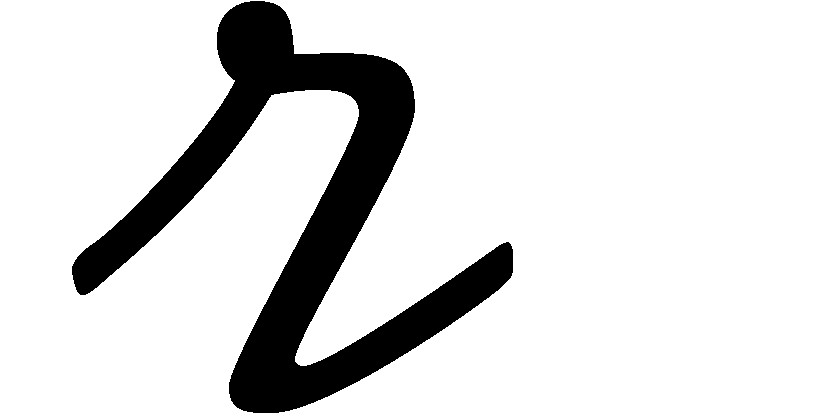
\includegraphics{ScriptR}}$}}}
\def\brcurs{{\mbox{$\resizebox{.16in}{.08in}{
\includegraphics{BoldR}}$}}}
\def\hrcurs{{\mbox{$\hat \brcurs$}}}
 
\begin{document}
\maketitle
\small
\section{Memory Bank}
\begin{enumerate}
\item Divergence and Curl of $\mathbf{B}$-fields, and current density:
\begin{align}
\nabla \cdot \mathbf{B} &= 0 \label{eq:0} \\
\nabla \times \mathbf{B} &= \mu_0 \mathbf{J} \label{eq:1} \\
I &= \int \mathbf{J} \cdot d\mathbf{a}
\end{align}
\end{enumerate}

\section{Calculating B-fields}

\begin{enumerate}
\item Take Equation \ref{eq:1} as a given, and perform a surface integral of both sides.  Let $I_{\rm enc}$ be the sum of currents that penetrate the surface.  (a) Use the curl theorem to show
\begin{equation}
\boxed{
\oint \mathbf{B} \cdot d\mathbf{l} = \mu_0 I
}
\end{equation} 
(b) Using Equation \ref{eq:0}, prove that $\mathbf{B}$-fields can have no monopole moment.  That is, there are no $\mathbf{B}$-fields like $\mathbf{B} = (B_0/r^2) \hat{\mathbf{r}}$.
\\ \vspace{2cm}
\item Consider the surface current density in Fig. \ref{fig:1} (left).  From dimensional analysis, we find that a surface current density times a distance equals a current (Fig. \ref{fig:1}, right).  Show that the corresponding $\mathbf{B}$-field is constant and in the $\hat{\mathbf{y}}$-direction, depending on the sign of $z$.
\end{enumerate}

\begin{figure}
\centering
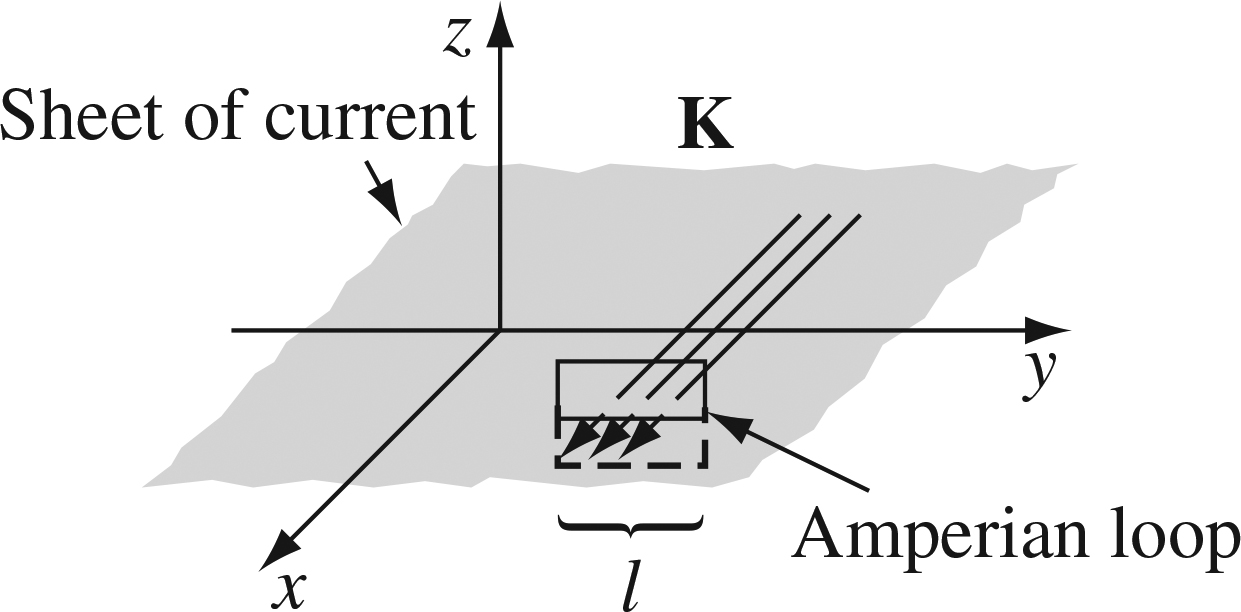
\includegraphics[width=0.45\textwidth]{figures/5_33.jpg}
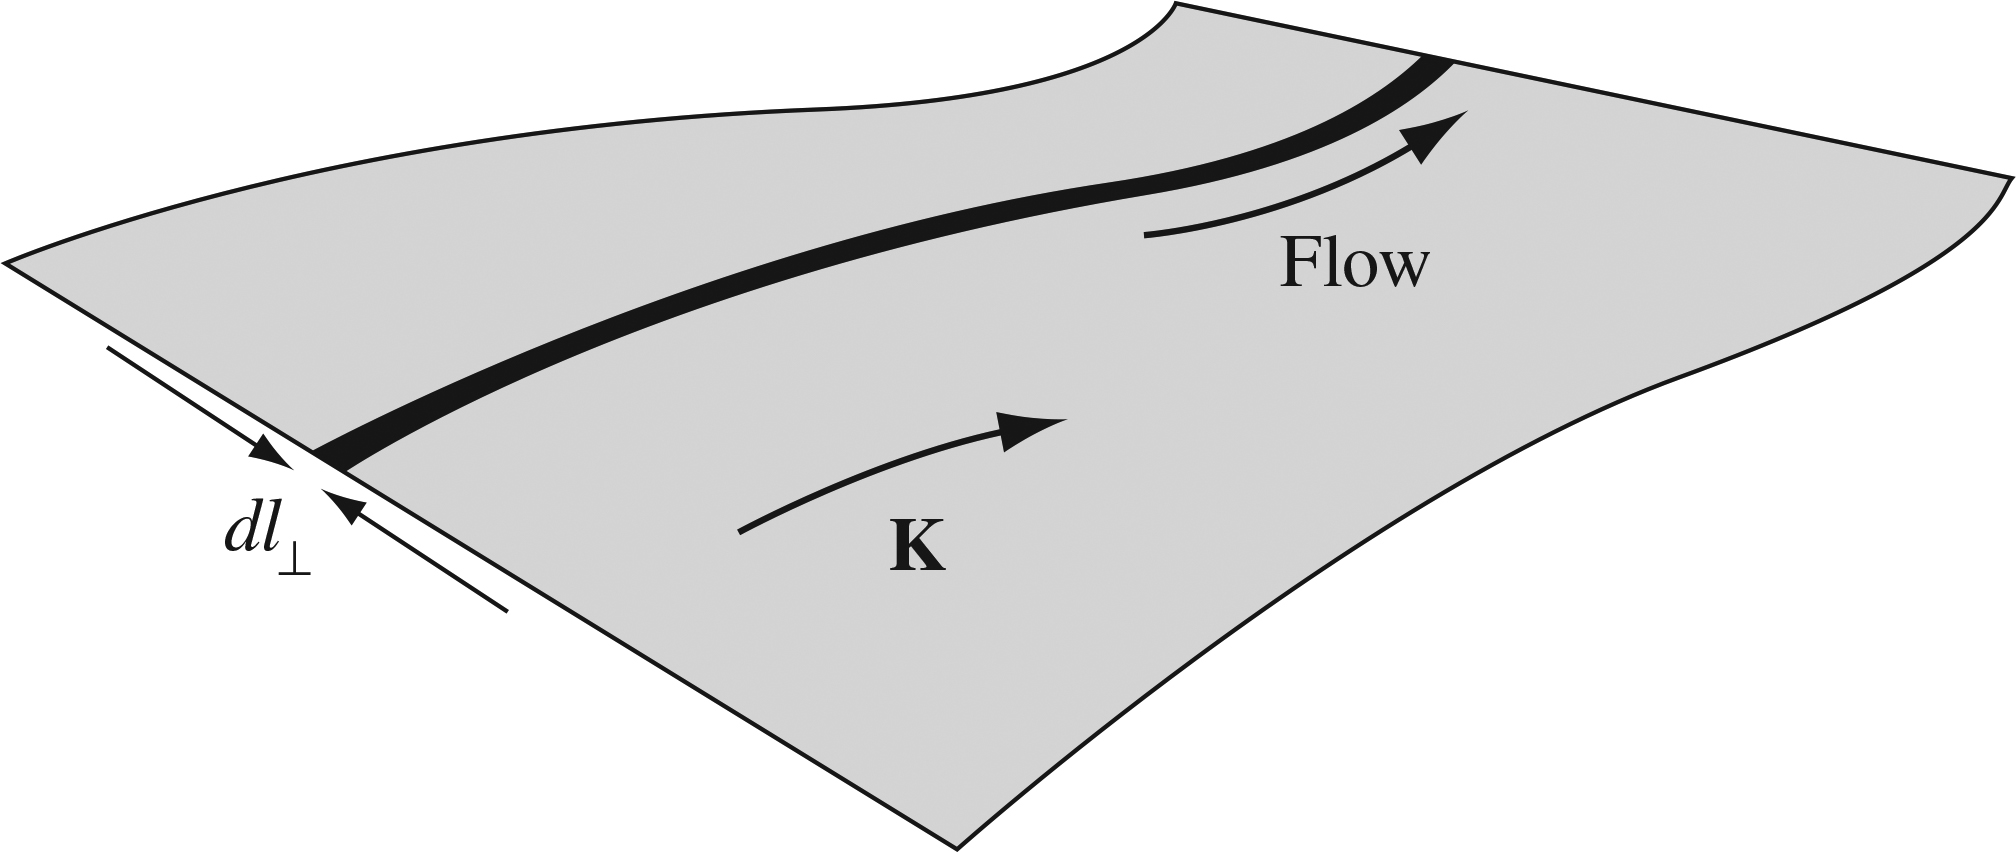
\includegraphics[width=0.45\textwidth]{figures/5_13.jpg}
\caption{\label{fig:1} (Left) An infinite uniform surface current density: $\mathbf{K} = K\hat{\mathbf{x}}$. (Right) A uniform surface current density times a distance $dl_{\perp}$ gives a current $dI$.}
\end{figure}

\end{document}